\documentclass[11pt,a4paper]{article}
\usepackage[T1]{fontenc}
\usepackage[utf8]{inputenc}
\usepackage{lmodern}
\usepackage{geometry}
\usepackage{graphicx}
\usepackage{booktabs}
\usepackage{array}
\usepackage{parskip}
\usepackage{hyperref}
\usepackage{xcolor}
\geometry{margin=24mm}
\graphicspath{{figures/}{../figures/}}
\definecolor{navy}{HTML}{19324E}
\hypersetup{colorlinks=true, urlcolor=navy, linkcolor=navy}
\setlength{\parindent}{0pt}

\begin{document}

\begin{titlepage}
  \centering
  \vspace*{34mm}
  {\Large\color{navy} TUNIS BUSINESS SCHOOL \par}
  \vspace{14mm}
  {\huge\bfseries Exploratory Data Analysis of\par}
  \vspace{2mm}
  {\huge\bfseries Credit Card Fraud Transactions\par}
  \vspace{10mm}
  {\large A Reproducible R Analysis and Portfolio Report\par}
  \vspace{24mm}
  {\Large\bfseries Jaouher Chouchane\par}
  \vspace{4mm}
  {\large Information Technology / Business Analytics\par}
  \vspace{4mm}
  BA 340 -- Data Analysis\par
  \vfill
  Individual Academic Project\par
  November 2025\par
\end{titlepage}

\section*{Abstract}

This project explores an anonymized credit card transaction dataset using R. It illustrates class imbalance, descriptive statistics, a stratified training/test partition, a comparison of transaction amounts, and two types of principal-component visualization. The analysis provides a reproducible workflow for calculating statistics from the source dataset. It does \emph{not} implement or evaluate a predictive fraud-detection model.

\section{Problem and objectives}

Fraud cases are rare relative to legitimate transactions. This makes data exploration important: a very small minority class may be difficult to see on plots or summarize with a single overall statistic.

The aims of this individual academic project are to:
\begin{itemize}
  \item describe class balance and transaction-amount distributions;
  \item demonstrate a reproducible stratified 70/30 split;
  \item visualize anonymized numerical features with PCA-related projections;
  \item demonstrate a statistical comparison of transaction amounts without claiming predictive ability.
\end{itemize}

\section{Dataset and preparation}

The dataset is the \href{https://www.kaggle.com/datasets/mlg-ulb/creditcardfraud}{Credit Card Fraud Detection dataset} published by the Machine Learning Group of the Universit\'e Libre de Bruxelles (ULB). The published dataset description reports \textbf{284,807 transactions}, including \textbf{492 fraud cases} (approximately \textbf{0.172\%}) and 284,315 legitimate cases. Transactions were recorded during two days in September 2013.

\begin{center}
\begin{tabular}{p{28mm} p{102mm}}
\toprule
\textbf{Column(s)} & \textbf{Meaning} \\
\midrule
\texttt{Class} & Fraud indicator: 1 = fraud, 0 = legitimate. \\
\texttt{Time} & Seconds elapsed since the dataset's first transaction; not a wall-clock timestamp. \\
\texttt{Amount} & Transaction amount. \\
\texttt{V1--V28} & Already anonymized and PCA-transformed numerical features. \\
\bottomrule
\end{tabular}
\end{center}

The R script checks required columns, missing values and invalid class labels, then creates an elapsed-hour bucket and a standardized transaction amount. The time bucket represents elapsed time modulo 24 hours, not the actual hour of day, because the dataset does not provide wall-clock timestamps.

\section{Methods}

\subsection{Descriptive statistics and stratified sampling}

The script computes the number and proportion of fraud and legitimate transactions, plus mean, median, standard deviation and quartiles of transaction amounts for each class. A deterministic 70/30 split is constructed separately within each class, preserving class proportions approximately. Since no prediction model is fitted, the split is a methodological demonstration rather than a train/test evaluation.

\subsection{Comparison of transaction amounts}

The code uses a \textbf{Welch two-sample t-test} to compare the mean transaction amounts, allowing unequal variances and very different group sizes. The program writes the actual statistic, p-value and confidence interval to \texttt{outputs/amount\_test.csv} when run.

Amount distributions can be skewed and contain extreme values, so results must be interpreted alongside medians and quartiles. A significant mean difference alone would not demonstrate a useful fraud detector.

\subsection{Principal component visualizations}

The first visualization plots \texttt{V1} against \texttt{V2}, features which have \emph{already} been PCA-transformed by the dataset creators. A second PCA on \texttt{V1--V28} serves as a teaching exercise in projection, \emph{not} as a recovery of confidential raw features or proof of predictability.

\section{Exploratory visualizations}

The figures illustrate exploratory patterns in the anonymized feature space. The R script also produces visualizations of class balance, feature distributions and transaction amounts when the dataset is provided.

\begin{figure}[htbp]
  \centering
  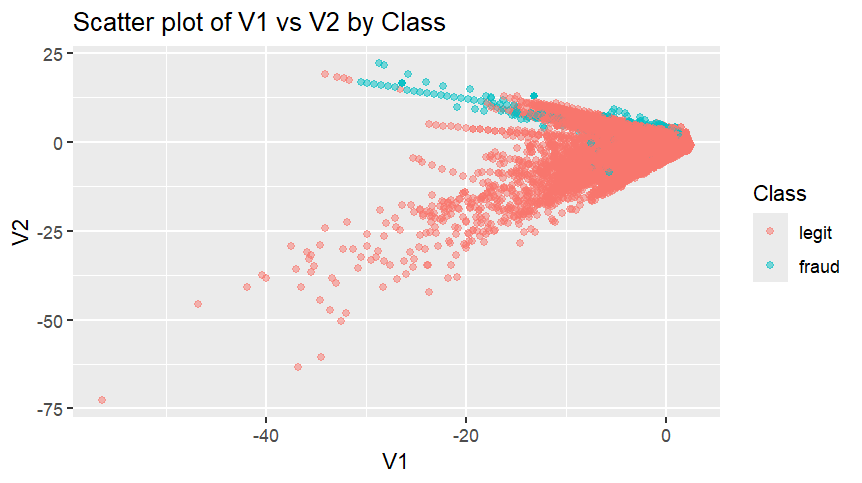
\includegraphics[width=0.92\linewidth]{v1_v2_scatter.png}
  \caption{V1/V2 scatter plot by class. The rare fraud class is visible among a much larger legitimate class.}
\end{figure}

\begin{figure}[htbp]
  \centering
  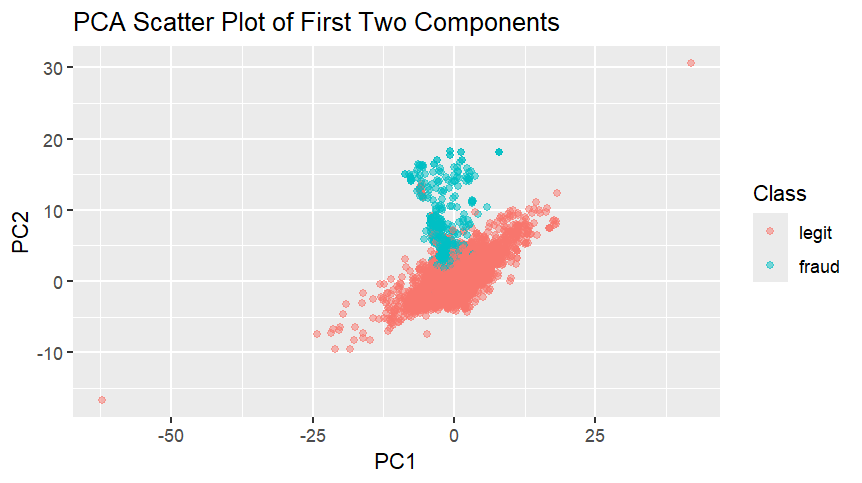
\includegraphics[width=0.92\linewidth]{secondary_pca_scatter.png}
  \caption{Secondary PCA projection of the already PCA-transformed variables. Overlap in projected points does not establish classification performance.}
\end{figure}

\clearpage
\section{Results and interpretation}

The published dataset's class balance can be stated accurately: only about 0.172\% of recorded transactions are labeled fraudulent. This imbalance matters for both visualization and any future machine-learning application.

The R script calculates class-specific amount summaries and a Welch t-test when \texttt{creditcard.csv} is supplied. This report does not assign numerical values to the test statistic, p-value or group means without an accompanying dataset execution.

The scatter plots suggest that some fraud observations occupy different regions of feature space, but the two-dimensional views also contain overlap and cannot quantify detection accuracy, false positives or recall. This report therefore makes no claims about a trained model or the statistical significance of the mean-amount difference.

\section{Limitations and future work}

\begin{itemize}
  \item Raw transaction features and cardholder identifiers are unavailable; the meaning of \texttt{V1--V28} cannot be recovered from this dataset.
  \item The dataset covers only two days of historical transactions, so generalization to current banking behavior cannot be assumed.
  \item Mean comparisons are sensitive to heavy-tailed transaction amounts; broader distributional analysis would be useful.
  \item The secondary PCA provides an alternate projection but does not add information about the confidential raw variables.
  \item No predictive classifier was trained. A future extension could compare logistic regression and random forests using a held-out test set and area under the precision-recall curve (AUPRC), which is more informative for rare fraud cases than accuracy alone.
\end{itemize}

\section{Reproducibility}

The analysis source code is provided in \texttt{analysis/analysis.R}. Download \texttt{creditcard.csv} from the dataset's publisher, install the R packages \texttt{data.table} and \texttt{ggplot2}, then run the command documented in \texttt{README.md}. The generated CSV tables and figures will appear in the ignored \texttt{outputs/} directory.

\textbf{Execution note:} The dataset is not bundled with the repository. Dataset-dependent statistical results are produced by running the R script locally; none are claimed in this report without verification.

\section*{References}

\begin{enumerate}
  \item Machine Learning Group, ULB. \emph{Credit Card Fraud Detection Dataset}. \url{https://www.kaggle.com/datasets/mlg-ulb/creditcardfraud}
  \item A. Dal Pozzolo, O. Caelen, R. A. Johnson, and G. Bontempi (2015). \emph{Calibrating Probability with Undersampling for Unbalanced Classification}. IEEE Symposium on Computational Intelligence and Data Mining.
\end{enumerate}

\end{document}
